% --- LaTeX Homework Template - S. Venkatraman ---

% --- Set document class and font size ---

\documentclass[letterpaper, 11pt]{article}

% --- Package imports ---

\usepackage{
  amsmath, amsthm, amssymb, mathtools, dsfont,	  % Math typesetting
  graphicx, wrapfig, subfig, float,                  % Figures and graphics formatting
  listings, color, inconsolata, pythonhighlight,     % Code formatting
  fancyhdr, sectsty, hyperref, enumerate, enumitem } % Headers/footers, section fonts, links, lists

% --- Page layout settings ---

% Set page margins
\usepackage[left=1.35in, right=1.35in, bottom=1in, top=1.1in, headsep=0.2in]{geometry}

% Anchor footnotes to the bottom of the page
\usepackage[bottom]{footmisc}
\usepackage{xcolor}
\usepackage{tikz}
\usepackage{pgfplots}

% Set line spacing
\renewcommand{\baselinestretch}{1}

% Set spacing between paragraphs
\setlength{\parskip}{1.5mm}

% Allow multi-line equations to break onto the next page
\allowdisplaybreaks

% Enumerated lists: make numbers flush left, with parentheses around them
\setlist[enumerate]{wide=0pt, leftmargin=21pt, labelwidth=0pt, align=left}
\setenumerate[1]{label={(\arabic*)}}

% --- Page formatting settings ---

% Set link colors for labeled items (blue) and citations (red)
\hypersetup{colorlinks=true, linkcolor=blue, citecolor=red}

% Make reference section title font smaller
\renewcommand{\refname}{\large\bf{References}}

% --- Settings for printing computer code ---

% Define colors for green text (comments), grey text (line numbers),
% and green frame around code
\definecolor{greenText}{rgb}{0.5, 0.7, 0.5}
\definecolor{greyText}{rgb}{0.5, 0.5, 0.5}
\definecolor{codeFrame}{rgb}{0.5, 0.7, 0.5}

% Define code settings
\lstdefinestyle{code} {
  frame=single, rulecolor=\color{codeFrame},            % Include a green frame around the code
  numbers=left,                                         % Include line numbers
  numbersep=8pt,                                        % Add space between line numbers and frame
  numberstyle=\tiny\color{greyText},                    % Line number font size (tiny) and color (grey)
  commentstyle=\color{greenText},                       % Put comments in green text
  basicstyle=\linespread{1.1}\ttfamily\footnotesize,    % Set code line spacing
  keywordstyle=\ttfamily\footnotesize,                  % No special formatting for keywords
  showstringspaces=false,                               % No marks for spaces
  xleftmargin=1.95em,                                   % Align code frame with main text
  framexleftmargin=1.6em,                               % Extend frame left margin to include line numbers
  breaklines=true,                                      % Wrap long lines of code
  postbreak=\mbox{\textcolor{greenText}{$\hookto$}\space} % Mark wrapped lines with an arrow
}

% Set all code listings to be styled with the above settings
\lstset{style=code}

% --- Math/Statistics commands ---

% Add a reference number to a single line of a multi-line equation
% Usage: "\numberthis\label{labelNameHere}" in an align or gather environment
\newcommand\numberthis{\addtocounter{equation}{1}\tag{\theequation}}

% Shortcut for bold text in math mode, e.g. $\b{X}$
\let\b\mathbf

% Shortcut for bold Greek letters, e.g. $\bg{\beta}$
\let\bg\boldsymbol

% Shortcut for calligraphic script, e.g. %\mc{M}$
\let\mc\mathcal

% \mathscr{(letter here)} is sometimes used to denote vector spaces
\usepackage[mathscr]{euscript}

% Convergence: right arrow with optional text on top
% E.g. $\converge[w]$ for weak convergence
\newcommand{\converge}[1][]{\xto{#1}}

% Normal distribution: arguments are the mean and variance
% E.g. $\normal{\mu}{\sigma}$
\newcommand{\normal}[2]{\mathcal{N}\left(#1,#2\right)}

% Uniform distribution: arguments are the left and right endpoints
% E.g. $\unif{0}{1}$
\newcommand{\unif}[2]{\text{Uniform}(#1,#2)}

% Independent and identically distributed random variables
% E.g. $ X_1,...,X_n \iid \normal{0}{1}$
\newcommand{\iid}{\stackrel{\smash{\text{iid}}}{\sim}}

% Equality: equals sign with optional text on top
% E.g. $X \equals[d] Y$ for equality in distribution
\newcommand{\equals}[1][]{\stackrel{\smash{#1}}{=}}

% Math mode symbols for common sets and spaces. Example usage: $\R$
\newcommand{\R}{\mathbb{R}}   % Real numbers
\newcommand{\C}{\mathbb{C}}   % Complex numbers
\newcommand{\Q}{\mathbb{Q}}   % Rational numbers
\newcommand{\Z}{\mathbb{Z}}   % Integers
\newcommand{\N}{\mathbb{N}}   % Natural numbers
\newcommand{\F}{\mathcal{F}}  % Calligraphic F for a sigma algebra
\newcommand{\El}{\mathcal{L}} % Calligraphic L, e.g. for L^p spaces

% Math mode symbols for probability
\newcommand{\pr}{\mathbb{P}}    % Probability measure
\newcommand{\E}{\mathbb{E}}     % Expectation, e.g. $\E(X)$
\newcommand{\var}{\text{Var}}   % Variance, e.g. $\var(X)$
\newcommand{\cov}{\text{Cov}}   % Covariance, e.g. $\cov(X,Y)$
\newcommand{\corr}{\text{Corr}} % Correlation, e.g. $\corr(X,Y)$
\newcommand{\B}{\mathcal{B}}    % Borel sigma-algebra

% Other miscellaneous symbols
\newcommand{\tth}{\text{th}}	% Non-italicized 'th', e.g. $n^\tth$
\newcommand{\Oh}{\mathcal{O}}	% Big-O notation, e.g. $\O(n)$
\newcommand{\1}{\mathds{1}}	% Indicator function, e.g. $\1_A$

% Additional commands for math mode
\DeclareMathOperator*{\argmax}{argmax}    % Argmax, e.g. $\argmax_{x\in[0,1]} f(x)$
\DeclareMathOperator*{\argmin}{argmin}    % Argmin, e.g. $\argmin_{x\in[0,1]} f(x)$
\DeclareMathOperator*{\spann}{Span}       % Span, e.g. $\spann\{X_1,...,X_n\}$
\DeclareMathOperator*{\bias}{Bias}        % Bias, e.g. $\bias(\hat\theta)$
\DeclareMathOperator*{\ran}{ran}          % Range of an operator, e.g. $\ran(T) 
\DeclareMathOperator*{\dv}{d\!}           % Non-italicized 'with respect to', e.g. $\int f(x) \dv x$
\DeclareMathOperator*{\diag}{diag}        % Diagonal of a matrix, e.g. $\diag(M)$
\DeclareMathOperator*{\trace}{trace}      % Trace of a matrix, e.g. $\trace(M)$

% Numbered theorem, lemma, etc. settings - e.g., a definition, lemma, and theorem appearing in that 
% order in Section 2 will be numbered Definition 2.1, Lemma 2.2, Theorem 2.3. 
% Example usage: \begin{theorem}[Name of theorem] Theorem statement \end{theorem}
\theoremstyle{definition}
\newtheorem{theorem}{Theorem}[section]
\newtheorem{proposition}[theorem]{Proposition}
\newtheorem{lemma}[theorem]{Lemma}
\newtheorem{corollary}[theorem]{Corollary}
\newtheorem{definition}[theorem]{Definition}
\newtheorem{example}[theorem]{Example}
\newtheorem{remark}[theorem]{Remark}

% Un-numbered theorem, lemma, etc. settings
% Example usage: \begin{lemma*}[Name of lemma] Lemma statement \end{lemma*}
\newtheorem*{theorem*}{Theorem}
\newtheorem*{proposition*}{Proposition}
\newtheorem*{lemma*}{Lemma}
\newtheorem*{corollary*}{Corollary}
\newtheorem*{definition*}{Definition}
\newtheorem*{example*}{Example}
\newtheorem*{remark*}{Remark}
\newtheorem*{claim}{Claim}

% --- Left/right header text (to appear on every page) ---

% Include a line underneath the header, no footer line
\pagestyle{fancy}
\renewcommand{\footrulewidth}{0pt}
\renewcommand{\headrulewidth}{0.4pt}

% Left header text: course name/assignment number
\lhead{Micro I - Assignment 2}

% Right header text: your name
\rhead{Zian Gong}

% --- Document starts here ---

\begin{document}

\textbf{Problem 11}

(1)

The preferences are continuous. Given a bundle $(x_1^*,x_2^*), x_1^*x_2^* = a$.

If $0<a<4$, then the $LCS = \{(x_1, x_2): x_1x_2 \leq a\}, UCS = \{(x_1,x_2) \geq a\}$. LCS and UCS are closed.

If $4 \leq a \leq 8$, then the $LCS = \{(x_1, x_2): x_1x_2 \leq 8\}, UCS = \{(x_1,x_2) \geq 4\}$. LCS and UCS are closed.

If $a > 8$, then the $LCS = \{(x_1, x_2): x_1x_2 \leq a\}, UCS = \{(x_1,x_2) \geq a\}$. LCS and UCS are closed.


(2)

$u(x_1,x_2)$ is quasi-concave. Let $(x_1, x_2) \gg 0$ and $(x_1',x_2') \gg 0$, we need to test a bundle if $u('\lambda x_1 + (1-\lambda)x_1',\lambda x_2, + (1-\lambda)x_2') \geq \min\{u(x_1,x_2), u(x_1',x_2')\}$, we can assume $x_1 \leq x_1', x_2 \leq x_2'$. \begin{align*}
     & [\lambda x_1 + (1-\lambda)x_1'] [\lambda x_2, + (1-\lambda)x_2']                        \\
     & = \lambda ^{2} x_1x_2 + \lambda(1-\lambda)[x_1'x_2 + x_1x_2'] + (1-\lambda)^{2}x_1'x_2' \\
     & \geq [\lambda ^{2} + 2\lambda(1-\lambda)+ (1-\lambda)^{2}]x_1x_2 = x_1x_2
\end{align*}

Since for function $u$, we have if $t_1t_2 \geq t_1't_2 \Longrightarrow u(t_1,x_2) \geq u(t_1',t_2')$, then \[
    u('\lambda x_1 + (1-\lambda)x_1',\lambda x_2, + (1-\lambda)x_2') \geq \min\{u(x_1,x_2), u(x_1',x_2')\}
\]
So $u(x_1,x_2)$ is quasi-concave.

\textcolor{red}{We cannot assume $x_1 \leq x_1', x_2 \leq x_2'$, but $x_1x_2 \leq x_1'x_2'$ is available.!
However, we can still get $x_1'x_2 + x_1x_2' \geq 2 \sqrt{x_1'x_2'x_1x_2} \geq 2 x_1x_2$.
}


(3)

$u(x_1,x_2)$ is not concave. For example, $u(1,1) = 1, u(2,2) = 4, u(3,3) = 9 \Longrightarrow u(2,2) < 0.5 u(1,1) + 0.5 u(3,3)$.

(4)

The utility function is not continuous. Check the point $(2,4), \forall \varepsilon > 0, \nexists \eta > 0$, such that if $\sqrt{(x-2)^{2} + (y-4)^{2}} < \eta, \text{then } \left| u(x,y) - 4 \right| < \varepsilon$.

Assume $x = 2+\eta/2, y = 4 + \eta/2$, then $xy = 8 + 3\eta + \frac{\eta ^{2}}{4} > 8$. We have \[
    u(x,y) = xy > 8 \Longrightarrow u(x,y) - u(2,4) > 4
\]
If $\varepsilon \leq 4$, it is impossible to find an $\eta$.

(5)

None of the previous statements contradict Debreu's theomem.

(6)

\[
    u(x_1,x_2) = \left\{\begin{array}{l}
        x_1x_2 \qquad \text{if } x_1x_2 \leq 4  \\
        4  \qquad \text{if } 4 \leq x_1x_2 < 8  \\
        x_1x_2 \qquad \text{if } x_1x_2  \geq 8 \\
    \end{array}\right.
\]
In this case, if $4 \leq x_1^*x_2^* < 8$, then the $LCS = \{(x_1, x_2): x_1x_2 < 8\}, UCS = \{(x_1,x_2) \geq 4\}$. LCS is open.

\bigskip
\hrule
\bigskip

\textbf{Problem 12}

(a) No, it is not complete. Because it does not define the preference when $h_1 > h_2 \wedge j_1 > j_2$. For example, situation 1: $j_1 = 5, h_1 = 5$; situation 2: $j_2 = 7, h_2 = 7$. The preference between $(5,5)$ and $(7,7)$ is not defined.

(b) Yes, it satisfies transitivity. $\forall (j_1,h_1) \in X, (j_2,h_2) \in X$ if $j_1 \geq j_2$, we have $(j_1,h_1) \succeq ((j_2,h_2))$, because $\geq $ is transitive, so this preference is transitive.

\textcolor{red}{NO. Counterexample: $(2,1), (3,7), (10,5)$\[
    (2,1) \sim (3,7), (3,7) \preceq (10,5), (2,1) \sim (10,5)
\]}

(c) No, it does not satisfy monotonicity. For counterexample, $(7,7) \sim (5,5)$ although $7>5$.

(d) Yes, it satisfies local non-satisfition. $\forall (j, h) \in X, \forall \varepsilon > 0, \exists \eta > 0,  \text{if } ||(j',h') - (j,h)|| < \eta$ then $(j',h') \succ (j,h) \iff j' - j > \varepsilon  \wedge h - h' > \varepsilon$. \[
    \sqrt{(j'-j)^{2} + (h'-h)^{2}} < \eta \Longrightarrow \left| j' -j \right| < \eta , \left| h'-h \right| < \eta
\]
Let $j' = j + \eta/2$ and $h'= h - \eta / 2 $, and let $\eta = 2\varepsilon$, we have \[
    j' - j > \varepsilon  \wedge h - h' > \varepsilon
\]

\bigskip
\hrule
\bigskip

\textbf{Problem 13}

\begin{figure}[H] % h=here, t=top, b=bottom, p=page
    \centering
    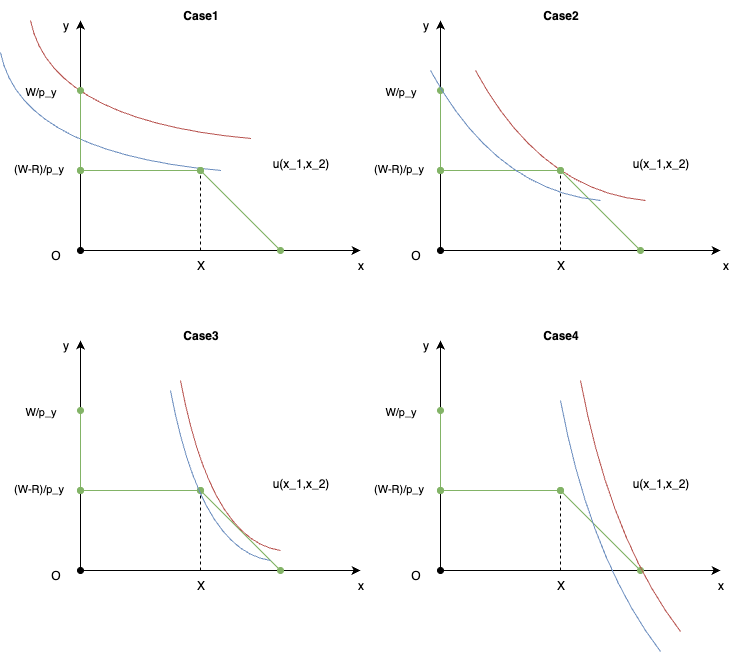
\includegraphics[width=0.8\textwidth]{images/micro1_ps1_p13.drawio.png}
    \caption{Problem 13: red indifference curves have higher utility}
    \label{fig:mylabel}
\end{figure}

\[
    p_x = \left\{\begin{array}{l}
        0 , \text{if } 0 \leq  x_1 \leq X \\
        p, \text{if } x_1 > X             \\
    \end{array}\right.
\]

According to figure \ref{fig:mylabel}, the green segments show the firms' budget constraints. And the decision of the firm depends on its indifference curve's shape.

Case1: the indifference curve is flat, the firm will not buy $x$.

Case2: the firm only buy $X$ units commodity $x$, and use surplus budget to buy $y$.

Case3: the firm buy more than $X$ units $x$ and some $y$, in this situation, the $MRS = p/p_y$.

Case4: the indifference curve is steep, the firm only by good $x$.

\textcolor{red}{Other cases}


\bigskip
\hrule
\bigskip

\textbf{Problem 14}


Assume commodities are $x_1, x_2$ respecting to their prices $p_1,p_2$, tax rate is $\alpha$, and given wealth is $w$. With proportional tax, the consumer's best choice bundle is $(x_1^*, x_2^*)$. According to budget constraints, we have \[
    (1+\alpha)p_1x_1^* + p_2x_2^* \leq w.
\]

The amount of total tax is $\alpha p_1 x_1^*$. When we change to wealth tax, the consumer's wealth is $w' = w - \alpha p_1 x_1^*$. Now we have a new budget constraint \[
    p_1x_1 + p_2x_2 \leq w - \alpha p_1 x_1^*.
\]

We can find that the commodity bundle $(x_1^*, x_2^*)$ can still be consumed in our new constraint. So, with wealth tax, the consumer can at least consume the same choice which maximizes his utility under proportional tax, which means it does not reduce consumer welfare.


\bigskip
\hrule
\bigskip

\textbf{Problem 20: MGW3.E.4}

(a) Show that if the consumer's preferences $\succeq $ are convex, then $h(p,u)$ is a convex set.


\begin{proof}
    If the $\succeq $ is convex, the $UCS = \{x \in X: x \succeq x^0\}$ is a convex set.

    Assume $u(x^0) = \bar{u}$.

    Let $H = h(p,\bar{u}) = \arg \min_{u(x) \geq \bar{u}} px$, we have \[
        \forall x \in H, u(x) \geq u(\bar{x^0}) = \bar{u}.
    \]

    Assume $x^1, x^2 \in H$, then $p x_1 = px_2 \leq px, \forall x \in \{x \in X: u(x) \geq \bar{u} \}$ and  $x^1, x^2 \in UCS$.

    Let $x^\lambda = \lambda x^1 + (1-\lambda)x^2, \lambda \in (0,1)$. Since $UCS$ is a convex set, then $x^\lambda \in UCS \iff u(x^\lambda) \geq \bar{u}$.

    And \[
        p x^\lambda = p \lambda x^1 +  p(1-\lambda)x^2 = \lambda px^1 = \lambda px^2.
    \]

    We have $px^\lambda = px^1 = px^2$ and $u(x^\lambda)\geq \bar{u}$, so $x^\lambda \in H$.

    $h(p,u)$ is a convex set.
\end{proof}



(b) Also show that if preferences are continuous and strictly convex, then $h(p,u)$ is single-valued.

\begin{proof}
    If the $\succeq $ is strictly convex, the $SUCS = \{x \in X: x \succ x^0\}$ is a convex set.

    Since the preferences are continuous, with Debreu's theorem, we know we can assume $u(\cdot )$ is continuous.

    \textbf{Existence}:

    $h(p,u)$ is a set of solution of program \begin{align*}
         & \min_{x \in X} \, px              \\
         & s.t.\, u(x) \geq u(x^0)
    \end{align*} $x$ is in a closed set.

    We can construct a new program \begin{align*}
         & \min_{x \in X} \, px              \\
         & s.t.\, \left\{\begin{array}{l}
             u(x) \geq u(x^0) \\
            p x \leq px^1, \, x^1 \in \{x \in X: px \geq px^0 \wedge u(x^1) \geq u(x^0)\} \\
         \end{array}\right.
    \end{align*}, now $x$ is in a compact set.

    With Weierstrass Theorem, we can know there exists a solution, so $h(p,u)$ is not empty.

    \textbf{Uniqueness}:

    By contradiction, we can assume $x^1, x^2 \in h(p,u), x^1 \neq x^2$, which means \[
        p x^1 = p x^2 \leq px,  \forall x \in \{x \in X: u(x) \geq u(x^0)\}
    \]
    and \[
        u(x^1) \geq u(x^0), \, u(x^2) \geq u(x^0).
    \]

    Let $x^\lambda = \lambda x^1 + (1-\lambda)x^2, \, \lambda \in (0,1)$, we have $px^\lambda = px^1 = px^2$, and since SUCS in a convex set, then we have \[
        u(x^\lambda) > u(x^0).
    \]

    Since $u(\cdot )$ is continuous, then $\exists \delta \in (0,1)$ such that $u(\delta x^\lambda) > u(x^0)$.

    However, \[
        p\delta x^\lambda < px^1 = px^2.
    \], it contradicts to the previous setting $p x^1 = p x^2 \leq px,  \forall x \in \{x \in X: u(x) \geq u(x^0)\}$.


    Conclusion, $h(p, u)$ is single valued.

\end{proof}


% --- Document ends here ---

\end{document}

